
\section{Related work}
\label{sec:relatedwork}

WebRTC enables real-time peer-to-peer communication between browsers
even in complex network settings with firewalls, proxies or Network
Address Translators (NAT). However, WebRTC manages neither addressing
nor routing. To establish a connection, two browsers need to exchange
offers and acknowledgments through a common mediator, e.g., mails,
dedicated signaling services~\cite{peerjs}, or existing WebRTC
connections~\cite{p}. Figure~\ref{fig:webrtcA} describes the very
first connection of one peer $p_1$ with another $p_2$ using a
signaling server. Figure~\ref{fig:webrtcB} shows instead that $p_3$
can later use $p_2$ as mediator instead of the signaling
service. Figure~\ref{fig:webrtcC} shows the resulting network. Note
that if $p_2$ crashes or leaves during the forwarding
process, the connection establishment will fail, even if
alternative routes exist as WebRTC does not manage routing.

% In Figure~\ref{fig:webrtcA}, $p_1$
% wants to connect to $p_2$. Therefore, $p_1$ pushes an offer ticket to a shared
% signaling service. It is worth noting that many signaling services can
% exist. Peer $p_2$ pulls the offer, stamps it and pushes it back to the signaling
% service. Finally, $p_1$ pulls the stamped ticket and establishes a bidirectional
% connection with $p_2$.  Identically, $p_3$ establishes a connection to $p_2$. We
% refer to the round-trip procedure as \emph{three-way handshake}. At this point,
% Peer $p_1$ is able to establish a connection to $p_3$ without the mediation of
% the former signaling service.  Instead, it uses $p_2$ as temporary signaling
% service.  As shown in Figure~\ref{fig:webrtcB}, Peer $p_1$ pushes an offer
% ticket to $p_2$. As $p_2$ is already connected to $p_3$, it forwards the offer
% to $p_3$ and registers $p_1$ as the emitter. Peer $p_3$ stamps the ticket and
% sends it back to $p_2$ who then forwards it back to $p_1$. Upon receipt, $p_1$
% establishes a bidirectional connection with $p_3$.  Notice that if $p_2$ crashes
% during the forwarding process, the connection establishment will fail, even if
% an alternative route exists as WebRTC does not manage routing.

Using signaling services and existing WebRTC connections makes it easy
to deploy random peer sampling protocols~\cite{jelasity2004peer} in
browsers that can run on mobile phones or tablets connected to mobile
networks~\cite{Carvajal-Gómez2015}. However, the complexity of the
WebRTC connection process further requires nodes to establish as few
connections as possible in order to reduce the generated traffic and
limit resource consumption. Unfortunately existing protocols fail at
this task.

Random peer sampling protocols~\cite{jelasity2004peer,jelasity2007gossip}
produce overlay networks by populating the partial views with references to
peers chosen at random among the network members following a uniform
distribution. Solely relying on local knowledge, they converge to a topology
exposing properties similar to those of random
graphs~\cite{erdos1959random}. Among others, they efficiently provide
connectedness and robustness. A wide variety of gossip-based protocols use
random peer sampling at their core. For instance, topology optimization
protocols~\cite{voulgaris2005epidemic,jelasity2009tman} aim at improving
localization, latency, or at addressing user preferences.

The representatives of random peer sampling protocols using a
fixed-size partial view comprise
Lpbcast~\cite{eugster2003lightweight},
HyParView~\cite{leitao2007hyparview}
Newscast~\cite{tolgyeski2009adaptive}, and
\CYCLON~\cite{voulgaris2005cyclon}. The developers deploying
applications using such protocols must foresee the dimensions of the
networks to setup properly their partial views size. These decisions
cannot be easily retracted afterwards at runtime. As a consequence,
applications tend to overestimate the required view sizes.

For example, a \CYCLON-based application may maintain 7 connections in
the browser despite requiring only 4. While this causes little harm in
standard IP-based networks. Maintaining too many active WebRTC
connections may uselessly overload a device. This calls for a dynamic
peer sampling service that can adapt to a dynamic number of
participants.

A way to achieve this adaptive behavior may consists in using one of
the several protocols for network-size estimation. For
example,~\cite{ganesh2007peer} samples and analyzes a subset of the
network and deduces the overall network size using probabilistic
functions.  Sketching techniques~\cite{baquero2012extrema} use instead
hashing to represent a large number of distinct node identities and
estimate the size of the using the resulting collisions in hash
values. Finally, averaging techniques~\cite{jelasity2004epidemic} use
aggregations that converge over exchanges to a value which depends on
the network size. Unfortunately, while they can be accurate in their
estimations, these approaches add a communication overhead which makes
them too expensive for mobile phones and similar devices.


% However, adaptiveness
% should introduce a minimum overhead to peer sampling
% protocols. % in WebRTC applications.

\begin{figure*}
  \centering
  \subfloat[Figure A][$p_1$ contacts $p_2$ to join the network. $p_1$ adds
  $p_2$ to its neighborhood. $p_1$ sends its request to $p_2$.]{
    
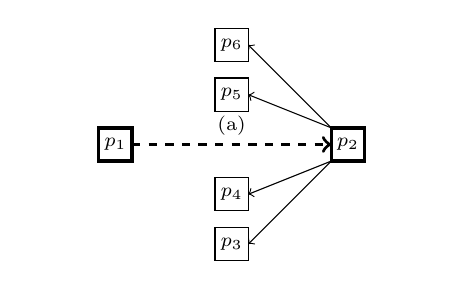
\begin{tikzpicture}[scale=1.2]

  \newcommand\X{35pt};
  \newcommand\Y{15pt};

  \draw(-0.75*\X, 0pt); %% positioning
  \draw( 2.75*\X, 0pt); %% positioning

  \scriptsize
  \draw[->,dashed,very thick](5+0*\X, 0*\Y) -- 
  node[anchor=south]{(a)}(-5+ 2*\X, 0*\Y);
  \draw[->] (-5+2*\X, 5pt) -- (5+\X, \Y);
  \draw[->] (-5+2*\X, 5pt) --  (5+\X, 2*\Y);
  \draw[->] (-5+2*\X, -5pt) -- (5+\X, -\Y);
  \draw[->] (-5+2*\X, -5pt) -- (5+\X, -2*\Y);

  \draw[fill=white, very thick]
  (0*\X, 0*\Y) node{$p_1$} +(-5pt,-5pt) rectangle +(5pt,5pt);
  \draw[fill=white, very thick]
  (2*\X, 0*\Y) node{$p_2$} +(-5pt,-5pt) rectangle +(5pt,5pt);

  \draw[fill=white](1*\X,2*\Y) node{$p_6$} +(-5pt,-5pt) rectangle +(5pt,5pt);
  \draw[fill=white](1*\X,1*\Y) node{$p_5$} +(-5pt,-5pt) rectangle +(5pt,5pt);
  \draw[fill=white](1*\X,-1*\Y) node{$p_4$} +(-5pt,-5pt) rectangle +(5pt,5pt);
  \draw[fill=white](1*\X,-2*\Y) node{$p_3$} +(-5pt,-5pt) rectangle +(5pt,5pt);
  
\end{tikzpicture}}
  \hspace{8pt}
  \subfloat[Figure B][The $onSubs(p_1)$ event is raised at $p_1$
  which forwards the subscription to $p_1$'s neighborhood.]{
    
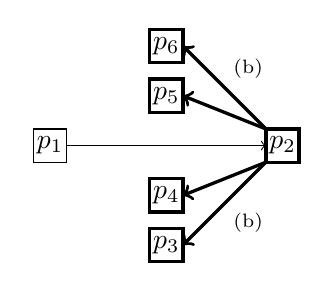
\begin{tikzpicture}[scale=1.2]

  \newcommand\X{35pt};
  \newcommand\Y{15pt};

  \scriptsize
  \draw[->](5+0*\X, 0*\Y) -- (-5+ 2*\X, 0*\Y);
  \draw[->, very thick] (-5+2*\X, 5pt) -- (5+\X, \Y);
  \draw[->, very thick] (-5+2*\X, 5pt) --
  node[anchor=south west]{(b)} (5+\X, 2*\Y);
  \draw[->, very thick] (-5+2*\X, -5pt) -- (5+\X, -\Y);
  \draw[->, very thick] (-5+2*\X, -5pt) --
  node[anchor=north west]{(b)}(5+\X, -2*\Y);

  \normalsize
  \draw[fill=white]
  (0*\X, 0*\Y) node{$p_1$} +(-5pt,-5pt) rectangle +(5pt,5pt);
  \draw[fill=white, very thick]
  (2*\X, 0*\Y) node{$p_2$} +(-5pt,-5pt) rectangle +(5pt,5pt);

  \draw[fill=white, very thick]
  (1*\X,2*\Y) node{$p_6$} +(-5pt,-5pt) rectangle +(5pt,5pt);
  \draw[fill=white, very thick]
  (1*\X,1*\Y) node{$p_5$} +(-5pt,-5pt) rectangle +(5pt,5pt);
  \draw[fill=white, very thick]
  (1*\X,-1*\Y) node{$p_4$} +(-5pt,-5pt) rectangle +(5pt,5pt);
  \draw[fill=white, very thick]
  (1*\X,-2*\Y) node{$p_3$} +(-5pt,-5pt) rectangle +(5pt,5pt);

\end{tikzpicture}}
  \hspace{8pt}
  \subfloat[Figure C][The $onFwdSubs(p_1)$ event is raised at $p_{3-6}$. The 
  peers add $p_1$ to their neighborhood.]{
    
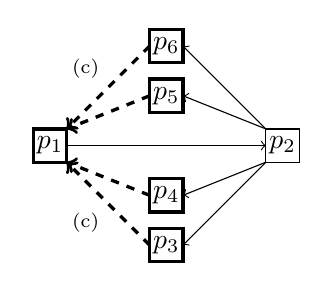
\begin{tikzpicture}[scale=1.2]

  \newcommand\X{35pt};
  \newcommand\Y{15pt};

  \scriptsize
  \draw[->](5+0*\X, 0*\Y) -- (-5+ 2*\X, 0*\Y);
  \draw[->] (-5+2*\X, 5pt) -- (5+\X, \Y);
  \draw[->] (-5+2*\X, 5pt) -- (5+\X, 2*\Y);
  \draw[->] (-5+2*\X, -5pt) -- (5+\X, -\Y);
  \draw[->] (-5+2*\X, -5pt) -- (5+\X, -2*\Y);

  \draw[->,dashed, very thick](-5+\X, 2*\Y) --
  node[anchor=south east]{(c)} ( 5pt,5pt);
  \draw[->,dashed, very thick](-5+\X, 1*\Y) -- ( 5pt,5pt);
  \draw[->,dashed, very thick](-5+\X, -1*\Y) -- ( 5pt,-5pt);
  \draw[->,dashed, very thick](-5+\X, -2*\Y) --
  node[anchor=north east]{(c)}( 5pt,-5pt);

  \normalsize
  \draw[fill=white, very thick]
  (0*\X, 0*\Y) node{$p_1$} +(-5pt,-5pt) rectangle +(5pt,5pt);
  \draw[fill=white]
  (2*\X, 0*\Y) node{$p_2$} +(-5pt,-5pt) rectangle +(5pt,5pt);

  \draw[fill=white, very thick]
  (1*\X,2*\Y) node{$p_6$} +(-5pt,-5pt) rectangle +(5pt,5pt);
  \draw[fill=white, very thick]
  (1*\X,1*\Y) node{$p_5$} +(-5pt,-5pt) rectangle +(5pt,5pt);
  \draw[fill=white, very thick]
  (1*\X,-1*\Y) node{$p_4$} +(-5pt,-5pt) rectangle +(5pt,5pt);
  \draw[fill=white, very thick]
  (1*\X,-2*\Y) node{$p_3$} +(-5pt,-5pt) rectangle +(5pt,5pt);
 

\end{tikzpicture}}
  \caption{\label{fig:joiningexample}Example of the \SPRAY's joining
    protocol.}
\end{figure*}

The sole representative of adaptive-by-design random peer sampling is
\SCAMP~\cite{ganesh2003peer}. Its interesting property lies in its
partial view sizes that grow logarithmically with the size of the
network. However, \SCAMP suffers from other drawbacks.
In particular, \SCAMP uses random walks to establish new connections
between peers. In WebRTC, each hop in these random paths must be
traveled back and forth to finalize the connection establishment
(cf. Figure~\ref{fig:webrtc}). This drastically increases the
probability that \SCAMP will fail in establishing connections. In the
presence of churn or message loss, the number of connections decreases
quickly,  eventually leading to network partitions
(cf. Section~\ref{subsec:degeneration}).

% The main point of criticism lies in it periodic
% balancing mechanism called \emph{lease}. After a while, each peer must join the
% network again. The arcs pointing to it are removed, and the peer chooses a
% neighbor from its untouched partial view to advertise its presence in the
% network. By doing so, it behaves as a newcomer which increases the number of
% arcs accordingly, despite it should not: the number of added arcs should be the
% exact number of removed arcs. Since all peers perform such mechanism on a
% regular basis, the number of arcs grows unbounded.  Also, 

% \SCAMP systematically disseminates the connections at random. Thus, the
% originating peer can be several hops away from the arrival peer. In WebRTC, each
% random dissemination path must be traveled back to finalize the connection
% establishment (cf. Figure~\ref{fig:webrtc}), often multiple times. This
% drastically impacts the \SCAMP failure probability of establishing a
% connection. In turns, the number of connections quickly decreases eventually
% leading to partitioning (cf. Section~\ref{subsec:degeneration}).


% Let $P_f$ be the probability that an
% element of the dissemination path (either a peer or a connection) crashes or
% leaves during a hop of the three-way handshake, without any possible
% recovery. Let $P_E$ be the probability that a connection establishment cannot
% be completed. Without three-way handshake, $P_E$ is straightforward:
% \begin{equation} P_{E,\,1way}^{Scamp}=1-(1- P_f)^{k+1} \end{equation} This
% corresponds to the probability that each element (arc and peer) in the path of
% size $k+1$ stays alive during their part of the dissemination (i.e., otherwise,
% they are allowed to crash or leave). In the context of WebRTC, the offer ticket must
% travel back to its emitter. As a consequence, the elements of the random
% dissemination path are not allowed to fail until the stamped ticket travels
% back. We obtain:
% \begin{align} P_{E,\,3way}^{Scamp} &=1 - ((1-P_f)^{2(k+1)} (1-P_f)^{2k}
%                                      \ldots (1-P_f)^2) \nonumber \\
%                                    &=1-(1-P_f)^{k^2+3k+2}
% \end{align}
% In other terms, the first chosen arc and peer in the path must stay alive $2k+2$
% hops, the second chosen arc and peer must stay alive $2k$ hops and so on.  The
% complexity class of the \SCAMP failure rate increases leading to a quicker
% degeneration of the connection count. This behavior endangers the network
% connectedness.%%, as depicted in Section~\ref{subsec:degeneration}.



%%% Local Variables:
%%% mode: latex
%%% TeX-master: "../paper"
%%% End:
